\documentclass[tikz,border=10pt]{standalone}

\begin{document}
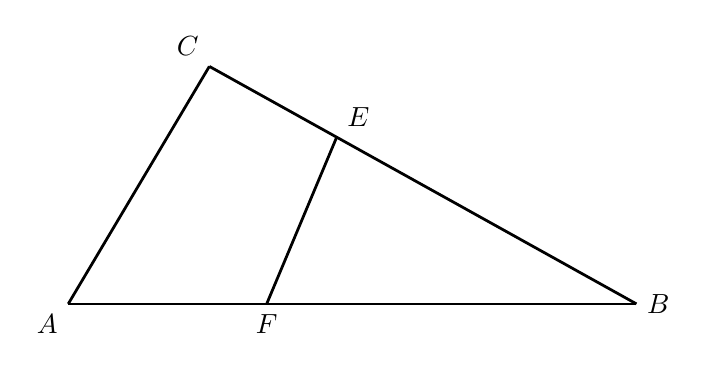
\begin{tikzpicture}[line join=round, line width=1.0pt]
\coordinate (A) at (-3.626,-1.499);
\coordinate (B) at (3.590,-1.499);
\coordinate (C) at (-1.834,1.517);
\coordinate (F) at (-1.106,-1.499);

  
  \coordinate (E) at (-0.217,0.618);

  
  \draw (A) -- (C);            
  \draw (C) -- (E) -- (B);     
  \draw (A) -- (F) -- (B);     

  
  \draw (F) -- (E);

  
  \node[below left]  at (A) {\fontsize{10}{12}\selectfont $A$};
  \node[right]       at (B) {\fontsize{10}{12}\selectfont $B$};
  \node[above left]  at (C) {\fontsize{10}{12}\selectfont $C$};
  \node[above right] at (E) {\fontsize{10}{12}\selectfont $E$};
  \node[below]       at (F) {\fontsize{10}{12}\selectfont $F$};
\end{tikzpicture}
\end{document}